% Preamble
%\documentclass[xetex,mathserif,serif]{beamer}
\documentclass{beamer}

% Packages
\usepackage[spanish]{babel}
\selectlanguage{spanish}
\usepackage[utf8]{inputenc} % For spanish (and international) letters like acents.
\usepackage{hyperref} % To create hyperlinks within the document.
\usepackage{graphicx} % To include graphics (pictures, images)
\usepackage{float} % For the use of the parameter "H" in command "\begin{figure}[H]" (i.e. exact position of image in text)
\usepackage{verbatim} % For long comments
\usepackage{tikz} % For include Dia diagrams in .tex format

\graphicspath{{../Diagramas/}} % Path of the folder containing the images

\title{Del código a la catalogación}
\subtitle{El sistema web para la catalogación y acceso de la colección de documentales del LAIS}
\author{Rodrigo Colín Rivera, Sergio Amaro Rosas}
\institute
{
  Laboratorio Audiovisual de Investigación Social\\
  Instituto de Investigaciones Dr. José María Luis Mora
}
\date{\today}
\subject{Catalogación de Colección de Documentales}

\begin{comment}
\AtBeginSection[]
{
  \begin{frame}
    \frametitle{Tabla de contenidos}
    \tableofcontents[currentsection]
  \end{frame}
}
\AtBeginSubsection[]
{
  \begin{frame}
    \frametitle{Tabla de contenidos}
    \tableofcontents[currentsection,currentsubsection]
  \end{frame}
}
\end{comment}

% Style and theme
\usetheme{PaloAlto}
%\usecolortheme{orchid} %crane,dolphin,lily

% Document environment
\begin{document}

\frame{\titlepage} % Página inicial

\section{Introducción}
\begin{frame}
	\frametitle{Introducción}
	Jornada sobre Documental e Investigación.
	
	En el marco del Día Mundial del Patrimonio Audiovisual.
\end{frame}

\section{Colección documental del LAIS}
\begin{frame}
	\frametitle{El LAIS}
	\framesubtitle{Colección documental del LAIS}
	
	El LAIS ha construido un acervo documental que se origina en 1993, año en que inicia la producción de su primer documental: \textit{Un pueblo en la memoria}.
	
	
\end{frame}

\section{Catalogación}
\begin{frame}
	\frametitle{Catalogación}
	\framesubtitle{Acerca de ISAD(G)}
	
	
\end{frame}

\section{Manual de Catalogación}
\begin{frame}
	\frametitle{Manual de Catalogación}
	\framesubtitle{Para el acervo documental en video del LAIS}
	
	
\end{frame}

\section{Situación y propuesta}
\begin{frame}
	\frametitle{Situación y Propuesta}
	\framesubtitle{¿Para qué catalogar?}
	
	
\end{frame}

\section{Sistema}
\begin{frame}
	\frametitle{El sistema}
	\framesubtitle{Esquema general}
	\begin{figure}[H]
		\centering
		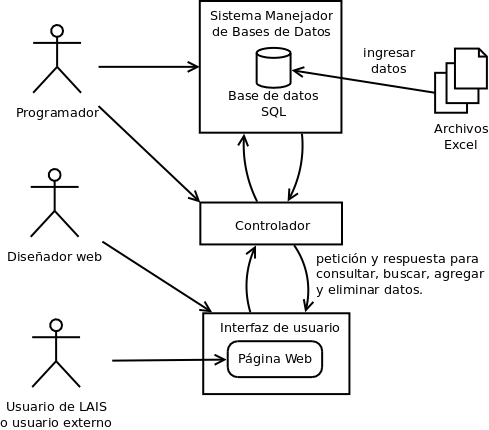
\includegraphics[width=0.7\textwidth]{EsquemaGeneral.png}
		\caption{Esquema general del sistema de consulta}
		\label{fig:esquema_general}
	\end{figure}
\end{frame}

\section{Requisitos}
\begin{frame}
	\frametitle{Requisitos a cumplir}
	\begin{figure}[H]
		\centering
		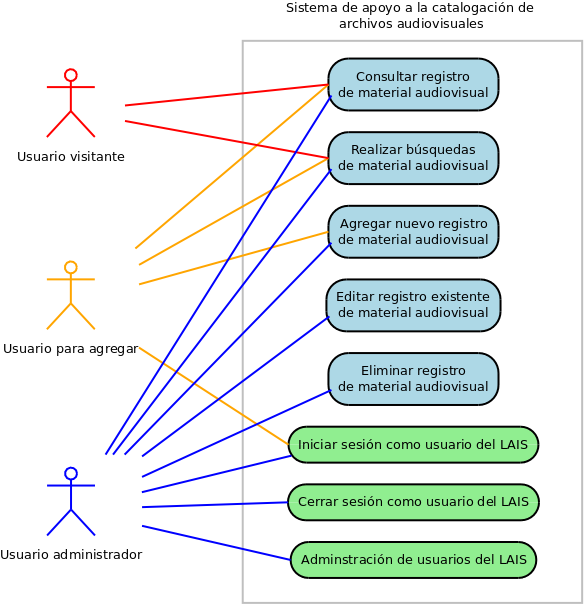
\includegraphics[width=0.6\textwidth]{CasosDeUso.png}
		\caption{Diagrama de casos de uso}
		\label{fig:caso_de_uso}
	\end{figure}
\end{frame}

\section{Acerca del desarrollo de software}
\begin{frame}
	\frametitle{Desarrollo de software}
	\framesubtitle{Consideraciones}
	Para el tipo de sistema que se desarrolló se tomo en cuenta los siguientes aspectos:
	\begin{itemize}
		\item Arquitectura Modelo-Vista-Controlador
		\item Sistema Manejador de Contenido
		\item Documentación asociada e ingeniería de software
	\end{itemize}
\end{frame}

\section{Demostración}
\begin{frame}
	\frametitle{Demostración}
	\framesubtitle{Primera versión del sistema}
	
	
\end{frame}

\section{Diseño}
\begin{frame}
	\frametitle{Acerca del diseño}
	\framesubtitle{Elementos visuales y de interacción con el usuario}
	
	
\end{frame}

\section{Conclusión}
\begin{frame}
	\frametitle{Conclusiones}
	\begin{itemize}
		\item Se logró implementar satisfactoriamente la parte principal del sistema que cumple con la arquitectura MVC y permite la administración completa de archivos audiovisuales y usuarios.
		\item Durante el desarrollo, siempre tener como objetivo la creación de un sistema capaz de organizarse y administrarse de manera simple por parte de los usuarios del LAIS sin la necesidad de intervención de los programadores.
		\item Crear y mantener una base de datos estandarizada para reutilizar esa información mediante un manejo semántico de contenido (siguiente proyecto a desarrollar).
	\end{itemize}
\end{frame}

\begin{frame}
	\begin{center}
		GRACIAS POR SU TIEMPO.
		
		%logo del LAIS
		%
\includegraphics{scientistapprovedfutura.png}
	\end{center}
\end{frame}

\end{document}